%Master File:lectures.tex

\lesson{Understand Mappings}
\vspace{-2cm}
\begin{center}
  \includegraphics[width=0.9\linewidth]{inverseProblem}
\end{center}
\keywords{Mappings, Eigenvectors}
%%%%%%%%%%%%%%%%%%%%%%% Next Slide %%%%%%%%%%%%%%%%%%%%%%%
\renewcommand{\Outline}{%
\begin{slide}
\section[1]{Outline}

\begin{minipage}{12cm}
  \begin{enumerate}\squeeze
    \outlineitem{Mappings}{mappings}
    \outlineitem{Linear Maps}{linearmaps}
    \outlineitem{Eigenvectors}{eigenvectors}
  \end{enumerate}
\end{minipage}\hfill
\begin{minipage}{10cm}
  \includegraphics[height=10cm]{ill_conditioned_map}
\end{minipage}
\end{slide}
\addtocounter{outlineitem}{1}
}

\setcounter{outlineitem}{1}
\Outline
\toptarget{firstoutline}
%%%%%%%%%%%%%%%%%%%%%%% Next Slide %%%%%%%%%%%%%%%%%%%%%%%

\begin{slide}
\section[-2]{Transforming Data}

\begin{PauseHighLight}
  \begin{itemize}
  \item In the last lecture we spent time developing a sophisticate view
    of vector spaces and operators\pause
  \item At a mathematical level machine learning can be viewed as
    performing an inverse mapping
    \begin{center}
      \includegraphics[width=12cm]{inverseProblem}\pause
    \end{center}
  \item Although our mappings are not necessarily linear in either
    direction we learn a lot by understanding linear operators\pause
  \end{itemize}
\end{PauseHighLight}



\end{slide}
%%%%%%%%%%%%%%%%%%%%%%% Next Slide %%%%%%%%%%%%%%%%%%%%%%%

\begin{slide}
\section{Inverse Problems}

\begin{PauseHighLight}
  \begin{itemize}
  \item Given $m$ observations $\{(\bm{x}_k, y_k)| k=1,\ldots,m\}$ and
    $p$ unknown $\bm{w}=(w_1,w_2, \ldots w_p)$ such that
    $\bm{x}_k^\tr \bm{w} = y_k$ then to find $\bm{w}$\pause
\item Define the \textit{design matrix} as the matrix of feature vectors
  \begin{displaymath}
    \mat{X} = 
    \begin{pmatrix}
      \bm{x}_1^\tr \\ \bm{x}_2^\tr \\ \hdots \\ \bm{x}_m^\tr
    \end{pmatrix} =
    \begin{pmatrix}
      x_{11} & x_{12} & \cdots & x_{1p}\\
      x_{21} & x_{22} & \cdots & x_{2p}\\
      \vdots & \vdots & \ddots & \vdots \\
      x_{m1} & x_{m2} & \cdots & x_{mp}
    \end{pmatrix}\pause
  \end{displaymath}
\item and the target vector $\bm{y} = (y_1, y_2, \cdots, y_m)^\tr$\pause
\item Then if $m=p$ we have $\bm{y} = \mat{X} \bm{w}$ or $\bm{w} =
  \mat{X}^{-1} \bm{y}$\pause
\end{itemize}

\end{PauseHighLight}
\end{slide}

%%%%%%%%%%%%%%%%%%%%%%% Next Slide %%%%%%%%%%%%%%%%%%%%%%%

\begin{slide}
\section[-2]{Linear Regression}

\pb
\begin{itemize}\squeeze
\item $y_k = \bm{x}_k^\tr \bm{w}$ depends on distance from separating
  plane\pauseh\pauselevel{=1}
\vspace*{-1cm}
\begin{center}
\multipdf[height=9.5cm]{linearRegression}\pause\\
\vspace*{-0.5cm}
\end{center}
\item If $m>p$ then $\mat{X}$ isn't square so doesn't have an inverse\pauseh
\item Worse unless the data is accurate $\bm{y} \approx \mat{X}
  \bm{w}\Rightarrow$ no ``solution''\pauseh
\item Problem solved by Gauss to predict the orbit of the asteroid Ceres\pauseh
\end{itemize}
\end{slide}

%%%%%%%%%%%%%%%%%%%%%%% Next Slide %%%%%%%%%%%%%%%%%%%%%%%

\begin{slide}
\section[-1.5]{Linear Least Squares}

\begin{PauseHighLight}

\begin{itemize}\squeeze
\item The error of input pattern $\bm{x}_k$ is
  \begin{displaymath}
    \epsilon_k  = \bm{x}_k^\tr \bm{w}-y_k\pause
  \end{displaymath}
\item The squared error
  \begin{displaymath}
    E(\bm{w}|\mathcal{D}) = 
    \sum_{k=1}^P\left(\bm{x}_k^\tr \bm{w}-y_k\right)^2
    = \sum_{k=1}^P \epsilon_k^2 = \| \bm{\epsilon} \|^2 \pause
  \end{displaymath}
\item We can define the error vector
  \begin{displaymath}
    \bm{\epsilon} = \mat{X} \bm{w} - \bm{y}
  \end{displaymath}
(note that $\epsilon_k = \bm{x}_k^\tr \bm{w} -y_k$)\pause
\item Minimising this error is known as the least squares problem\pause
\end{itemize}

\end{PauseHighLight}
\end{slide}

%%%%%%%%%%%%%%%%%%%%%%% Next Slide %%%%%%%%%%%%%%%%%%%%%%%

\begin{slide}
\section[-2]{Finding a Minimum}

\begin{PauseHighLight}
  \begin{itemize}
  \item The minima of a one dimensional function, $f(x)$, are given by
    $f'(x)=0$
    \begin{center}
      \includegraphics[width=0.5\linewidth]{gradient}\pause
    \end{center}
  \item The minima of an $n$-dimensions function $f(\bm{x})$ are
    given by the set of equations
    \begin{align*}
      \frac{\partial f(\bm{x})}{\partial x_i}=0 
      \quad \forall i=1,\ldots n\pause
    \end{align*}
  \end{itemize}
\end{PauseHighLight}

\end{slide}

%%%%%%%%%%%%%%%%%%%%%%% Next Slide %%%%%%%%%%%%%%%%%%%%%%%

\begin{slide}
  \section[-1]{Gradients}

  \begin{PauseHighLight}

    \begin{itemize}
    \item The \emph{grad} operator $\grad$ is the gradient operator in
      high dimensions
      \begin{displaymath}
        \grad f(\bm{x}) = 
        \begin{pmatrix}
          \frac{\partial f(\bm{x})}{\partial x_1} \\
          \frac{\partial f(\bm{x})}{\partial x_2} \\
          \vdots \\
          \frac{\partial f(\bm{x})}{\partial x_n}
        \end{pmatrix}\pause
      \end{displaymath}
    \item The partial derivatives (curly d's)
      \begin{displaymath}
        \frac{\partial f(\bm{x})}{\partial x_i}
      \end{displaymath}
      means differentiate with respect to $x_i$ treating all other components
      $x_j$ as constants\pause
    \end{itemize}

  \end{PauseHighLight}
\end{slide}

%%%%%%%%%%%%%%%%%%%%%%% Next Slide %%%%%%%%%%%%%%%%%%%%%%%

\begin{slide}
\section[-2]{Least Squares Solution}

\begin{PauseHighLight}

\begin{itemize}\squeeze
\item The least squared solution is give by
  \begin{align*}
    \grad E(\bm{w}|\mathcal{D}) &= \grad \|\bm{\epsilon}\|^2 \pause
    = \grad \| \mat{X} \bm{w} - \bm{y}\|^2 \pause \\
    &= \grad \left(\bm{w}^\tr
      \mat{X}^\tr\mat{X} \, \bm{w} -  2 \bm{w}^\tr\mat{X}^\tr \bm{y} +
      \bm{y}^\tr  \bm{y}\right)\pause\\
    &= 2 \left( \mat{X}^\tr\mat{X}\, \bm{w} - \mat{X}^\tr
      \bm{y}\right)\pause = 0 \pause
  \end{align*}
\item Or
  \begin{displaymath}
    \bm{w} = \left(\mat{X}^\tr\mat{X}\right)^{-1} \mat{X}^\tr \bm{y}\pause
    = \mat{X}^{+} \bm{y}
  \end{displaymath}
\item $\mat{X}^{+} = \left(\mat{X}^\tr\mat{X}\right)^{-1} \mat{X}^\tr$ is
  known as the pseudo inverse\pause
\item For non-square matrices Matlab uses the pseudo inverse so in
  Matlab we can write
  \begin{matlab}
    w = X\y
  \end{matlab}\pause
\end{itemize}

\end{PauseHighLight}
\end{slide}


%%%%%%%%%%%%%%%%%%%%%%% Next Slide %%%%%%%%%%%%%%%%%%%%%%%
\Outline % Linear Maps
%%%%%%%%%%%%%%%%%%%%%%% Next Slide %%%%%%%%%%%%%%%%%%%%%%%

\begin{slide}
\section{Solving Inverse Problems}

\begin{PauseHighLight}
  \begin{itemize}
  \item Gauss showed us how to solve \emph{over-constrained} problems
    (we have more observations than parameters)\pause
  \item We seek a solution which isn't necessarily exact but minimises
    an error\pause
  \item But, what if we have more parameters than observations\pause
  \item That is, we are \emph{under-constrained}\pause
  \item Note that in some directions you might be over-constrained and
    in other directions under-constrained\pause
  \item This is very typical of most machine learning problems\pauseb
  \end{itemize}
\end{PauseHighLight}

\end{slide}

%%%%%%%%%%%%%%%%%%%%%%% Next Slide %%%%%%%%%%%%%%%%%%%%%%%

\begin{slide}
\section[-2]{Under Constrained Systems}

\begin{PauseHighLight}
  \begin{itemize}
  \item If we have less data-points than parameters then there will be
    multiple solutions
  \begin{center}
    \includegraphics[height=12cm]{curves}\pause
  \end{center}
  \end{itemize}
\end{PauseHighLight}

\end{slide}


%%%%%%%%%%%%%%%%%%%%%%% Next Slide %%%%%%%%%%%%%%%%%%%%%%%

\begin{slide}
\section[-2]{What is the Inverse?}

\pb
  \begin{itemize}
  \item Many points can map to the same points\pause
    \begin{center}
      \includegraphics[width=0.75\linewidth]{underConstrained0}\mypl{1}
      \llap{\includegraphics[width=0.75\linewidth]{underConstrained1}}\mypl{2}
    \end{center}
  \end{itemize}

\end{slide}

%%%%%%%%%%%%%%%%%%%%%%% Next Slide %%%%%%%%%%%%%%%%%%%%%%%

\begin{slide}
\section[-1]{Under-constrained Systems}

\begin{PauseHighLight}
  \begin{itemize}
  \item The system is \emph{under-constrained}\pause
  \item We have more unknowns than equations\pause
  \item The inverse is not unique\pause
  \item Solving the inverse problem ($\bm{w} =
    \left(\mat{X}^\tr\mat{X}\right)^{-1} \mat{X}^\tr \bm{y}$) is said 
    to be \emph{ill-posed}\pause
  \item The inverse $\left(\mat{X}^\tr\mat{X}\right)^{-1}$ doesn't
    exist\pause 
  \item If we have a complicated learning machine and not sufficient
    data we often end with an ill-posed inverse problem (there are lots
    of sets of parameters that explain the data)\pause
  \end{itemize}
\end{PauseHighLight}

\end{slide}


%%%%%%%%%%%%%%%%%%%%%%% Next Slide %%%%%%%%%%%%%%%%%%%%%%%

\begin{slide}
  \section{Ill-Conditions}

  \begin{PauseHighLight}
    \begin{itemize}
    \item Singular matrices are rare (although they occur when we don't
      have enough data), but matrices that are close to
      being singular are common\pause
    \item If a matrix is close to singular it is ill-conditioned\pause
    \item Ill-conditioned matrices have some small eigenvalues\pause
    \item All points get contracted towards a plane\pause
    \item Large matrices are very often ill conditioned\pause
    \end{itemize}
  \end{PauseHighLight}
\end{slide}

%%%%%%%%%%%%%%%%%%%%%%% Next Slide %%%%%%%%%%%%%%%%%%%%%%%

\begin{slide}
  \section[-1]{Ill-Conditioned Matrices}

  \begin{PauseHighLight}

    \begin{center}
      \includegraphics[height=15cm]{ill_conditioned_map}
    \end{center}

  \end{PauseHighLight}
\end{slide}

%%%%%%%%%%%%%%%%%%%%%%% Next Slide %%%%%%%%%%%%%%%%%%%%%%%

\begin{slide}
\section{Ill-Conditioning in ML}

\begin{PauseHighLight}
  \begin{itemize}
  \item Ill-conditioning in machine learning occurs when a very small
    change in the learning data causes a large change in the predictions
    of the learning machine\pause
  \item In linear regression the matrix $\mat{X}^\tr\mat{X}$ is
    ill-conditioned when we have as many data points as parameters\pause
  \item Much of machine learning is concerned with making learning
    machines better conditioned\pause
  \item Adding regularisers is one approach to achieve this\pause
  \end{itemize}
\end{PauseHighLight}

\end{slide}

%%%%%%%%%%%%%%%%%%%%%%% Next Slide %%%%%%%%%%%%%%%%%%%%%%%
\Outline % Eigenvectors
%%%%%%%%%%%%%%%%%%%%%%% Next Slide %%%%%%%%%%%%%%%%%%%%%%%

\begin{slide}
\section[-2]{Eigenvalue equation}
\pb

  \begin{itemize}
  \item Eigen-systems help us to understand mappings\pauseh
  \item A vector $\bm{v}$ is said to be an \emph{eigenvector} if
    \begin{minipage}{0.5\linewidth}
      \begin{displaymath}
        \mat{M} \bm{v} = \lambda \, \bm{v}\pauseh
      \end{displaymath}
    \end{minipage}\hfill
    \begin{minipage}{0.4\linewidth}
      \multipdf[height=7cm]{eigenvector}\pause
    \end{minipage}
  \item $\mat{M}$ is square (i.e. $n\stimes n$)\pauseh
  \item Where the number $\lambda$ is the \emph{eigenvalue}\pauseh
  \item Eigenvalues play a fundamental role in understanding operators\pauseh
  \end{itemize}


\end{slide}


%%%%%%%%%%%%%%%%%%%%%%% Next Slide %%%%%%%%%%%%%%%%%%%%%%%

\begin{slide}
\section[-1]{Symmetric Matrices}

\begin{PauseHighLight}
  \begin{itemize}
  \item If $\mat{M}$ is an $n\stimes n$ \emph{symmetric} matrix then it has
    $n$ real orthogonal eigenvectors with real eigenvalues\pause
  \item We denote the $i^{th}$ eigenvector by $\bm{v}_i$ and the
    corresponding eigenvalue by $\lambda_i$ so that
    \begin{displaymath}
      \mat{M} \bm{v}_i = \lambda_i \, \bm{v}_i \pause
    \end{displaymath}
  \item Orthogonal means that if $i\neq j$ then
    \begin{displaymath}
      \bm{v}_i^\tr \, \bm{v}_j = 0\pause
  \end{displaymath}
  \item (We can always normalise eigenvectors if we want)\pause
  \end{itemize}
\end{PauseHighLight}

\end{slide}


%%%%%%%%%%%%%%%%%%%%%%% Next Slide %%%%%%%%%%%%%%%%%%%%%%%

\begin{slide}
\section[-2]{Proof of Orthogonality}

\begin{PauseHighLight}
  \begin{itemize}
  \item $\left(\strut \mat{M}\bm{v}_i = \lambda_i\bm{v}_i\right)^\tr$
    implies $\bm{v}_i^\tr \mat{M}^\tr = \lambda_i\bm{v}_i^\tr$\pause
  \item When $\mat{M}$ is symmetric then $\mat{M}\bm{v}_i = \lambda_i\bm{v}_i
    \Rightarrow \bm{v}_i^\tr \mat{M} = \lambda_i\bm{v}_i^\tr$\pause
  \item Consider two eigenvectors $\bm{v}_i$ and $\bm{v}_j$ of $\mat{M}$
    \begin{align*}
      \bm{v}_i^\tr \mat{M} \bm{v}_j &= (\bm{v}_i^\tr \mat{M}) \bm{v}_j =
      \lambda_i  \bm{v}_i^\tr \bm{v}_j \\
      &= \bm{v}_i^\tr (\mat{M} \bm{v}_j)
      = \lambda_j  \bm{v}_i^\tr \bm{v}_j\pause
    \end{align*}
  \item So either $\lambda_i = \lambda_j$ or $\bm{v}_i^\tr \bm{v}_j=0$\pause
  \item If $\lambda_i = \lambda_j$ then any vector in the plane spanned
    by $\bm{v}_i$ and $\bm{v}_j$ are eigenvectors and we can always
    choose two orthogonal vectors in the plane\pause
  \end{itemize}
\end{PauseHighLight}

\end{slide}


%%%%%%%%%%%%%%%%%%%%%%% Next Slide %%%%%%%%%%%%%%%%%%%%%%%

\begin{slide}
\section[-2]{Orthogonal Matrices}

\begin{PauseHighLight}
  \begin{itemize}
  \item We can construct an \emph{orthogonal} matrix $\mat{V}$ from the
    eigenvectors
    \begin{displaymath}
      \mat{V} = (\bm{v}_1, \bm{v}_2 , \cdots, \bm{v}_n)\pause
    \end{displaymath}
    \vspace*{-1cm}
  \item Matrix $\mat{V}$ is an $n\stimes n$ matrix\pause
  \item Because of the orthogonality of the vectors $\bm{v}_i$
    \begin{displaymath}
      \mat{V}^\tr \, \mat{V} \pause =
      \begin{pmatrix}
        \bm{v}^\tr_1 \bm{v}_1 & \bm{v}^\tr_1 \bm{v}_2 & \cdots &
        \bm{v}^\tr_1 \bm{v}_n
        \\
        \bm{v}^\tr_2 \bm{v}_1 & \bm{v}^\tr_2 \bm{v}_2 & \cdots &
        \bm{v}^\tr_2 \bm{v}_n
        \\
        \vdots & \vdots & \ddots & \vdots
        \\
        \bm{v}^\tr_n \bm{v}_1 & \bm{v}^\tr_n \bm{v}_2 & \cdots &
        \bm{v}^\tr_n \bm{v}_n
      \end{pmatrix} \pause =
      \begin{pmatrix}
        1 & 0 & \cdots & 0 \\
        0 & 1 & \cdots & 0 \\
        \vdots & \vdots & \ddots & \vdots \\
        0 & 0 & \cdots & 1
      \end{pmatrix} \pause
      = \mat{I}\pause
    \end{displaymath}
  \end{itemize}
\end{PauseHighLight}

\end{slide}

%%%%%%%%%%%%%%%%%%%%%%% Next Slide %%%%%%%%%%%%%%%%%%%%%%%

\begin{slide}
\section[-2]{The Other Way Around}

\begin{PauseHighLight}
  \begin{itemize}
  \item We have shown that $\mat{V}^\tr \, \mat{V} = \mat{I}$\pause
  \item Thus multiply both sides on the left by $\mat{V}$
    \begin{align*}
      \mat{V}\,\mat{V}^\tr \, \mat{V} = \mat{V}\pause
    \end{align*}
  \item $\mat{V}$ will have an inverse,
    $\mat{V}^{-1}$, such that
    $\mat{V} \, \mat{V}^{-1} = \mat{I}$\pause
  \item Multiplying the equation on the right by $\mat{V}^{-1}$
    \begin{align*}
      (\mat{V}\,\mat{V}^\tr) \, \mat{V} \, \mat{V}^{-1}
      &= \mat{V}\,\mat{V}^{-1}\pause  \\
      \mat{V}\,\mat{V}^\tr &= \mat{I}\pauseb
    \end{align*}
  \item Note that, $\mat{V}^{-1}=\mat{V}^\tr$ (definition of
    orthogonal matrix)\pause
  \end{itemize}
\end{PauseHighLight}

\end{slide}

%%%%%%%%%%%%%%%%%%%%%%% Next Slide %%%%%%%%%%%%%%%%%%%%%%%

\begin{slide}
\section[-2]{Invertible Matrices}

\begin{PauseHighLight}
  \begin{itemize}
  \item A matrix, $\mat{M}$, will be singular (uninvertible) if there
    exists a vector $\bm{x}$ ($\neq\bm{0}$) such that
    \begin{align*}
      \mat{M}\,\bm{x} = \bm{0}\pause
    \end{align*}
  \item Now if there exists such a vector such that $\mat{V}\,\bm{x} =
    \bm{0}$ then multiply by $\mat{V}^\tr$ we get
    \begin{align*}
      \mat{V}^\tr\, \mat{V}\, \bm{x} &= \mat{V}^\tr\, \bm{0} \pause \\
      \bm{x} &= \bm{0}
    \end{align*}
    since $\mat{V}^\tr\, \mat{V} = \mat{I}$\pauseb
  \item Thus $\bm{V}$ is invertible\pauseb
  \end{itemize}
\end{PauseHighLight}

\end{slide}



%%%%%%%%%%%%%%%%%%%%%%% Next Slide %%%%%%%%%%%%%%%%%%%%%%%

\begin{slide}
\section[-2]{Rotations}

\begin{PauseHighLight}
  \begin{itemize}
  \item Orthogonal matrices satisfy $\mat{V}^\tr \mat{V} = \mat{V}\,
    \mat{V}^\tr=\mat{I}$\pause
  \item As a consequent they define rotations (and possibly a reflection)\pause
  \item Consider a vector $\bm{x}$ and $\bm{x}'=\mat{V}\bm{x}$, now
    \begin{align*}
      \| \bm{x}' \|_2^2 = \bm{x}^{\prime\tr}\bm{x}'\pause
      = (\mat{V}\bm{x})^\tr (\mat{V}\bm{x})\pause
      = \bm{x}^\tr \mat{V}^\tr \mat{V} \bm{x}\pause
      = \bm{x}^\tr \bm{x} \pause = \| \bm{x} \|_2^2 \pause
    \end{align*}
  \item Similarly if additionally $\bm{y}'=\mat{V}\bm{y}$ then
    {\small
    \begin{align*}
      \langle \bm{x}', \bm{y}' \rangle = (\mat{V}\bm{x})^\tr
      (\mat{V}\bm{y})\pause
       = \bm{x}^\tr \mat{V}^\tr \mat{V} \bm{y}\pause
       = \bm{x}^\tr \bm{y} \pause = \langle \bm{x}, \bm{y} \rangle\pause
       = \| \bm{x} \|_2 \, \| \bm{y} \|_2 \, \cos(\theta)\pause
    \end{align*}}
  \item Rotations and reflections preserve lengths and angles\pause
  \end{itemize}
\end{PauseHighLight}

\end{slide}

%%%%%%%%%%%%%%%%%%%%%%% Next Slide %%%%%%%%%%%%%%%%%%%%%%%

\begin{slide}
\section[-2]{Matrix Decomposition}

\begin{PauseHighLight}
  \begin{itemize}
  \item Taking the matrix of eigenvectors, $\bm{V}$, then
    \begin{align*}
      \mat{M}\, \mat{V}  &= \mat{M} (\bm{v_1},\bm{v}_2,\ldots,\bm{v}_n)\pause
      =
      (\lambda_1\,\bm{v_1},\lambda_2\,\bm{v}_2,\ldots,\lambda_n\,\bm{v}_n)\pause
      = \mat{V} \,\mat{\Lambda}\pause
    \end{align*}
  \item where $\mat{\Lambda} = \mathrm{diag}(\lambda_1,
    \lambda_2,\ldots, \lambda_n) =
    \begin{pmatrix}
      \lambda_1 & 0 & \cdots & 0 \\
      0 & \lambda_2  & \cdots & 0 \\
      \vdots & \vdots &\ddots &\vdots \\
      0 & 0 & \cdots & \lambda_n
    \end{pmatrix}$\pause
  \item Now
    \begin{align*}
      \mat{M} = \mat{M}\, \mat{V} \, \mat{V}^\tr = \mat{V}
      \,\mat{\Lambda} \, \mat{V}^\tr \pause
    \end{align*}
  \item Very important \textit{similarity transform}\pause
  \end{itemize}
\end{PauseHighLight}

\end{slide}


%%%%%%%%%%%%%%%%%%%%%%% Next Slide %%%%%%%%%%%%%%%%%%%%%%%

\begin{slide}
\section[-2]{Mappings by Symmetric Matrices}

\pb \pause
\begin{center}
  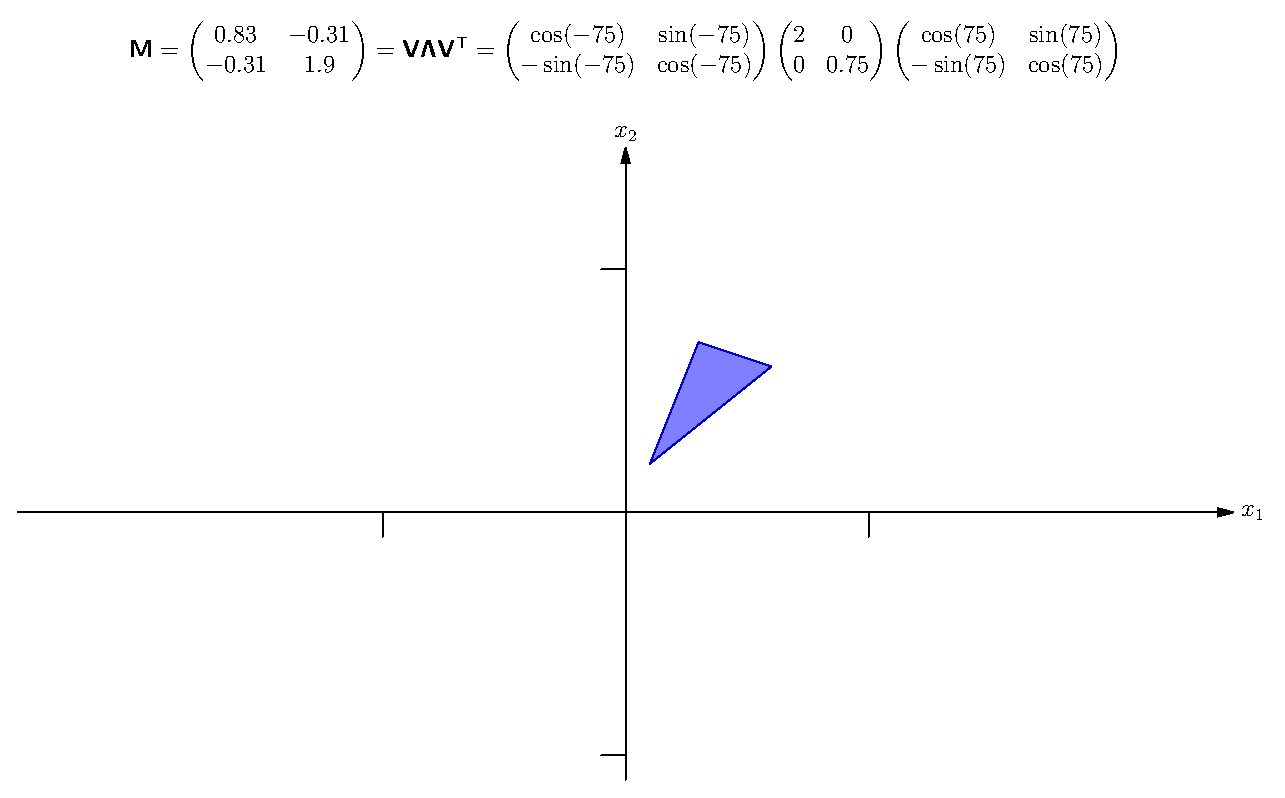
\includegraphics[width=\linewidth]{symmatrixPicture1}\mypl{1}
  \multido{\i=2+1}{7}{%
    \llap{\includegraphics[width=\linewidth]{symmatrixPicture\i}}\mypl{\i}}
\end{center}
\end{slide}


%%%%%%%%%%%%%%%%%%%%%%% Next Slide %%%%%%%%%%%%%%%%%%%%%%%

\begin{slide}
\section[-2]{Inverses}

\begin{PauseHighLight}
  \begin{itemize}
  \item For any square matrix
    \begin{align*}
      \mat{M} &=\mat{V}\,\mat{\Lambda}\,\mat{V}^\tr \pause &
      \mat{M}^{-1} &=\mat{V}\,\mat{\Lambda}^{-1}\,\mat{V}^\tr \pause 
    \end{align*}
  \item Where $\mat{\Lambda}^{-1} = \diag(\tfrac{1}{\lambda_1},
    \tfrac{1}{\lambda_2}, \ldots, \tfrac{1}{\lambda_n}) =
    \begin{pmatrix}
      \tfrac{1}{\lambda_1} & 0 & \cdots & 0 \\
      0 & \tfrac{1}{\lambda_2}  & \cdots & 0 \\
      \vdots & \vdots &\ddots &\vdots \\
      0 & 0 & \cdots & \tfrac{1}{\lambda_n}
    \end{pmatrix}$\pause
  \item Since
    \begin{align*}
       \mat{M}\,\mat{M}^{-1} &= (\mat{V}\,\mat{\Lambda}\,\mat{V}^\tr)\,
       (\mat{V}\,\mat{\Lambda}^{-1}\,\mat{V}^\tr)\pause
       = \mat{V}\,\mat{\Lambda}\,(\mat{V}^\tr\,
       \mat{V})\,\mat{\Lambda}^{-1}\,\mat{V}^\tr)\pause \\
       &= \mat{V}\,\mat{\Lambda}\,\mat{\Lambda}^{-1}\,\mat{V}^\tr\pause
       = \mat{V}\,\mat{V}^\tr = \mat{I}\pause
    \end{align*}
  \item I.e, Small eigenvalues become large eigenvalues and visa verse\pause
  \end{itemize}
\end{PauseHighLight}

\end{slide}

%%%%%%%%%%%%%%%%%%%%%%% Next Slide %%%%%%%%%%%%%%%%%%%%%%%

\begin{slide}
\section[-1.5]{Ill-Conditioning Again}

\pb\pause\pauselevel{=1}
\begin{center}
  \multipdf[width=0.9\linewidth]{conditioning}\pause
\end{center}

\end{slide}

%%%%%%%%%%%%%%%%%%%%%%% Next Slide %%%%%%%%%%%%%%%%%%%%%%%

\begin{slide}
\section[-2]{Condition Number}

\begin{PauseHighLight}
  \begin{itemize}\squeeze
  \item Taking matrix inverses can be inherently unstable\pause
  \item Any small error can be amplified by taking the inverse\pause
  \item The stability of the inverse depends on the ratio of smallest
    eigenvalue to the largest eigenvalue (i.e. the biggest possible
    amplification compared to the smallest)\pause
  \item Note that the Hilbert-norm of a matrix is the absolute value of
    the largest eigenvalue\pause
  \item The condition number is given by
    \begin{align*}
      \|\mat{M}\|_H \times \|\mat{M}^{-1}\|_H =
      \frac{|\lambda_{\text{\small max}}|}{|\lambda_{\text{\small min}}|}\pause
    \end{align*}
  \item Large condition number implies very ill-conditioned\pause
  \end{itemize}
\end{PauseHighLight}

\end{slide}



%%%%%%%%%%%%%%%%%%%%%%% Next Slide %%%%%%%%%%%%%%%%%%%%%%%

\begin{slide}
\section{Summary}

\begin{PauseHighLight}
  \begin{itemize}
  \item Linear mappings are commonly used in machine learning algorithms
    such as regression\pause
  \item We will often meet the pseudo-inverse involving inverting
    $\mat{X}^\tr\,\mat{X}$\pause 
  \item They can be inherently unstable to noise in the inputs\pause
  \item We can understand symmetric operators by looking at their eigenvectors\pause
  \item Function spaces can similarly be understood in terms of eigenfunctions\pause
  \end{itemize}
\end{PauseHighLight}

\end{slide}


%%% Local Variables:
%%% TeX-master: "lectures"
%%% End:
